\documentclass{beamer}
\usepackage{notation}
\usepackage{forloop}
\usepackage{hyperref}

\usetheme{metropolis}           % Use metropolis theme
\title{Gaussian Processes}
\date{\today}
\author{Nipun Batra}
\institute{IIT Gandhinagar}
\begin{document}
  \maketitle
  
  
  
\section{Gaussian Distribution}
  \begin{frame}{1d Gaussian Scatter Plot}
    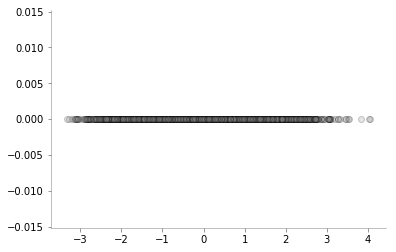
\includegraphics[width=\linewidth,height=\textheight,keepaspectratio]{gp/1d-gp}
  \end{frame}

  \begin{frame}{1d Gaussian Histogram}
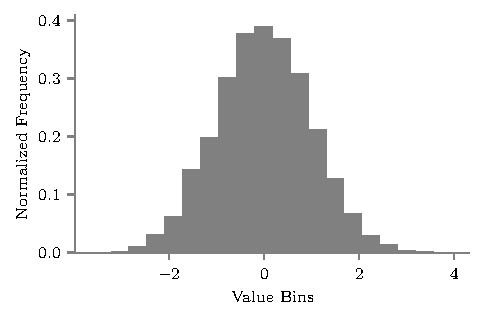
\includegraphics[width=\linewidth,height=\textheight,keepaspectratio]{gp/1d-gp-hist}
\end{frame}

  \begin{frame}{Varying 1d Gaussian Variance}
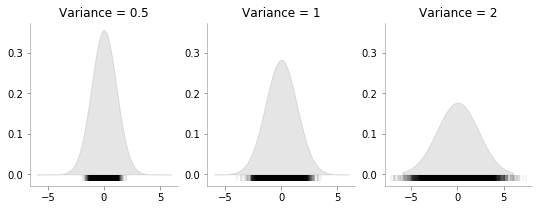
\includegraphics[width=\linewidth,height=\textheight,keepaspectratio]{gp/1d-gp-kde2}\end{frame}

\begin{frame}{Bi-variate Gaussian}
$$
\begin{pmatrix}
X_1 \\
X_2
\end{pmatrix}  \sim \mathcal{N} \left( \begin{pmatrix}
\mu_1 \\
\mu_2
\end{pmatrix} , \begin{pmatrix}
a &\rho \\
\rho & b
\end{pmatrix} \right)
$$
\end{frame}

\begin{frame}{Sampling Bi-variate Gaussian - 1}
\begin{center}
	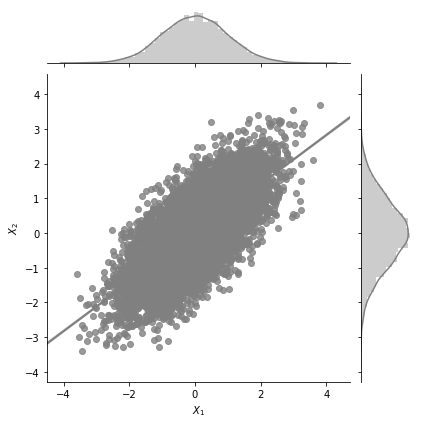
\includegraphics[height=\textheight -10pt ,keepaspectratio]{gp/2d-gp}
\end{center}
\end{frame}


\begin{frame}{Sampling Bi-variate Gaussian - 2}
	\begin{center}
		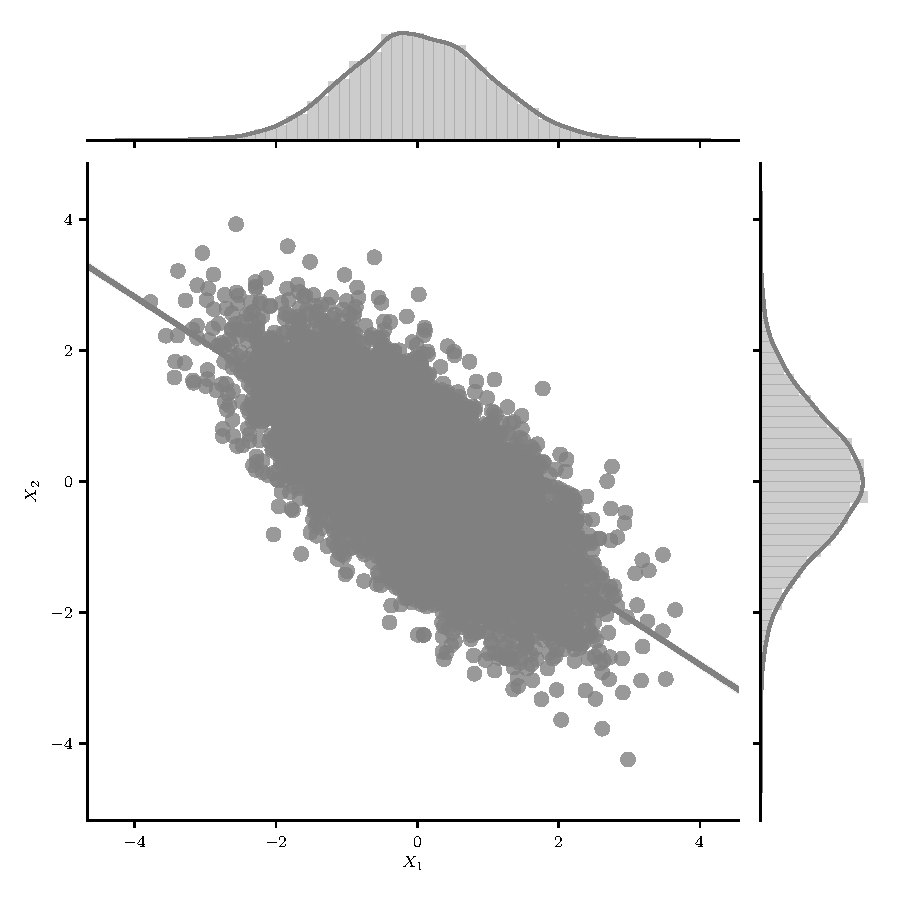
\includegraphics[height=\textheight -10pt ,keepaspectratio]{gp/2d-gp2}
	\end{center}
\end{frame}

\begin{frame}{Sampling Bi-variate Gaussian - 3}
	\begin{center}
		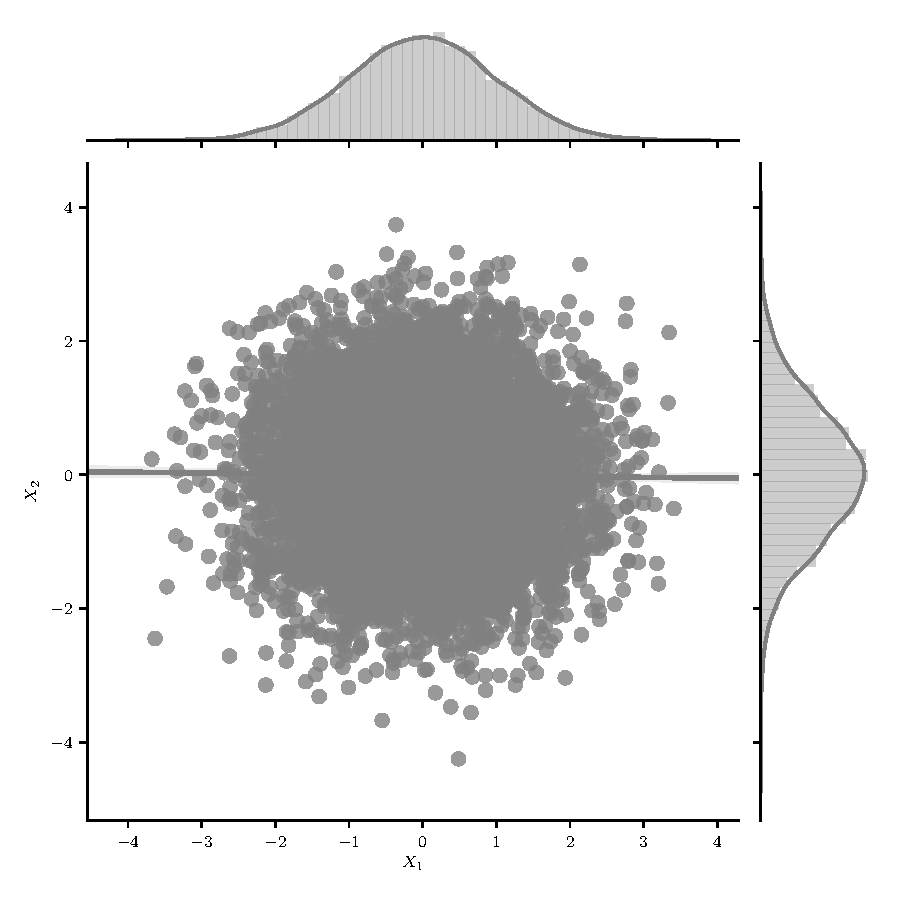
\includegraphics[height=\textheight -10pt ,keepaspectratio]{gp/2d-gp3}
	\end{center}
\end{frame}

\begin{frame}{Surface Plots Bi-variate Gaussian - 1}
	\begin{center}
		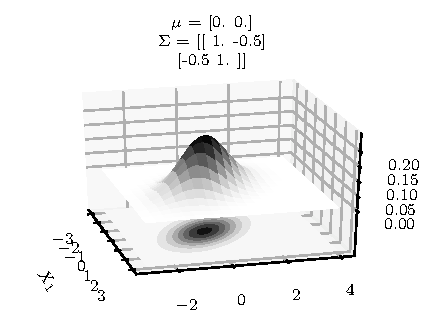
\includegraphics[height=\textheight -10pt ,keepaspectratio]{gp/2dgp3d}
	\end{center}
\end{frame}

\begin{frame}{Surface Plots Sampling Bi-variate Gaussian - 2}
	\begin{center}
		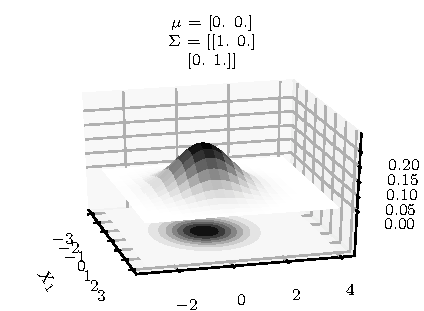
\includegraphics[height=\textheight -10pt ,keepaspectratio]{gp/2dgp3d2}
	\end{center}
\end{frame}

\section{Visualizing samples from 2d Gaussian}

% for cov
\newcounter{iter}
\forloop{iter}{1}{\value{iter} < 6}%
{%
	\begin{frame}{Cov = 0.1 | Random State - \theiter}
		\includegraphics[width=\linewidth,height=\textheight,keepaspectratio]{gp/0.1/\theiter}
	\end{frame}
}
% for cov
\forloop{iter}{1}{\value{iter} < 6}%
{%
	\begin{frame}{Cov = 0.7 | Random State - \theiter}
		\includegraphics[width=\linewidth,height=\textheight,keepaspectratio]{gp/0.7/\theiter}
	\end{frame}
}

\section{Conditional Bi-variate Distribution}

\begin{frame}{Conditional Bi-variate Distribution}
$$
\begin{pmatrix}
	X_1 \\
	X_2
\end{pmatrix}  \sim \mathcal{N} \left( \begin{pmatrix}
	0 \\
	0
\end{pmatrix} , \begin{pmatrix}
	1 & \rho \\
	\rho & 1
\end{pmatrix} \right)
$$

The conditional expectation of $X_2$ given $X_1$ is: $\operatorname{E}(X_2 \mid X_1=x_1)= \rho x_1$

and the conditional variance is: $\operatorname{var}(X_2 \mid X_1 = x_1) = 1-\rho^2$
\end{frame}

% for cov
\forloop{iter}{1}{\value{iter} < 6}%
{%
	\begin{frame}{Conditional bi-variate | Cov = 0.1 | Random State - \theiter}
		\includegraphics[width=\linewidth,height=\textheight,keepaspectratio]{gp/conditional/0.1/\theiter}
	\end{frame}
}

% for cov
\forloop{iter}{1}{\value{iter} < 6}%
{%
	\begin{frame}{Conditional bi-variate | Cov = 0.7 | Random State - \theiter}
		\includegraphics[width=\linewidth,height=\textheight,keepaspectratio]{gp/conditional/0.7/\theiter}
	\end{frame}
}

\section{5D Multivariate}

% for cov
\forloop{iter}{1}{\value{iter} < 6}%
{%
	\begin{frame}{Multivariate Gaussian Sample | Random State - \theiter}
		\begin{center}
			\includegraphics[width=\linewidth, height=\textheight -120pt ,keepaspectratio]{gp/5d/\theiter}
		\end{center}
		From the visualisation above we can see that:
		\begin{itemize}
			\item Since $X_1$ and $X_2$ are highly correlated, they move up and down together
			\item but, $X_1$ and $X_5$ have low correlation, thus, they can seem to wiggle almost independently of each other.
		\end{itemize}
	\end{frame}
}

\section{Conditional Multivariate Distribution}

\urldef\urlwik\url{https://en.wikipedia.org/wiki/Multivariate\_normal\_distribution#Conditional\_distributions}

\label{sec:condMul}
\begin{frame}{Conditional Multivariate Distribution Definition\footnote{\urlwik}}
	If $N$-dimensional $\vecMat{x}$ is partitioned as follows
	$$\mathbf{x}
	=
	\begin{bmatrix}
	\mathbf{x}_A \\
	\mathbf{x}_B
	\end{bmatrix}
	\text{ with sizes }\begin{bmatrix} q \times 1 \\ (N-q) \times 1 \end{bmatrix}$$
	and accordingly $\vecMat{\mu}$ and $\vecMat{\Sigma}$ are partitioned as follows
	$$\boldsymbol\mu
	=
	\begin{bmatrix}
		\boldsymbol\mu_A \\
		\boldsymbol\mu_B
	\end{bmatrix}
	\text{ with sizes }\begin{bmatrix} q \times 1 \\ (N-q) \times 1 \end{bmatrix}$$
	$$\boldsymbol\Sigma
	=
	\begin{bmatrix}
	\boldsymbol\Sigma_{AA} & \boldsymbol\Sigma_{AB} \\
	\boldsymbol\Sigma_{BA} & \boldsymbol\Sigma_{BB}
	\end{bmatrix}
	\text{ with sizes }\begin{bmatrix} q \times q & q \times (N-q) \\ (N-q) \times q & (N-q) \times (N-q) \end{bmatrix}$$	
\end{frame}

\begin{frame}
	then the distribution of $\mathbf{x}_A$ conditional on $\mathbf{x}_B = \vecMat{b}$ is multivariate normal $(\vecMat{x}_A|\vecMat{x}_B=b)\sim \mathcal{N}(\bar{\vecMat{\mu}}, \bar{\vecMat{\Sigma}})$
	$$\bar{\boldsymbol\mu}
	=
	\boldsymbol\mu_A + \boldsymbol\Sigma_{AB} \boldsymbol\Sigma_{BB}^{-1}
	\left(
	\mathbf{B} - \boldsymbol\mu_B
	\right)$$
	and covariance matrix
	$$\overline{\boldsymbol\Sigma}
	=
	\boldsymbol\Sigma_{AA} - \boldsymbol\Sigma_{AB} \boldsymbol\Sigma_{BB}^{-1} \boldsymbol\Sigma_{BA}.$$
	
\end{frame}

% for cov
\forloop{iter}{1}{\value{iter} < 6}%
{%
	\begin{frame}{Conditional Multivariate Distribution | Random State - \theiter}
		\begin{center}
			\includegraphics[width=\linewidth, height=\textheight -120pt ,keepaspectratio]{gp/5d/conditional/1/\theiter}
		\end{center}
		From the visualisation above we can see that:
		\begin{itemize}
			\item Since $X_4$ and $X_5$ are highly correlated, $X_4$ moves such that it's value is similar to the fixed value of $X_5$.
			\item but, $X_1$ and $X_5$ have low correlation, thus, there seems low relation between the values of these points.
		\end{itemize}
	\end{frame}
}

\begin{frame}{20 Dimensional Multivariate}
	\begin{center}
		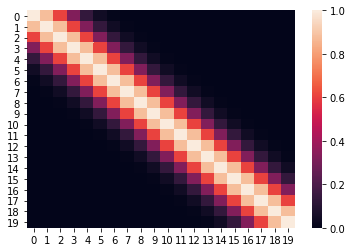
\includegraphics[width=\linewidth, height=\textheight -120pt ,keepaspectratio]{gp/20d}\\
	\end{center}	
	The above heatmap shows that there is correlation between nearby points, but close to zero or zero correlation otherwise.
\end{frame}

% for cov
\forloop{iter}{1}{\value{iter} < 6}%
{%
	\begin{frame}{Multivariate (20D) Distribution Samples | Random State - \theiter}
		\begin{center}
			\includegraphics[width=\linewidth, height=\textheight -120pt ,keepaspectratio]{gp/20d/\theiter}
		\end{center}
		From the animation above, we can see different family of functions of mean zero across 20 points. Notice that nearby points are more correlated (making the curve smooth) than the points farther away.
	\end{frame}
}

\begin{frame}{Adding new Data Points}
	Now we want to update the model with new data. We find the functional value at the points $X_1, X_2, X_6, X_11$.
	
	We will be using the equations at the start of \hyperref[sec:condMul]{section} Conditional multivariate distribution, to update or Guassian Process, in the wake of new data points.
\end{frame}

\begin{frame}{Updated Covariance Matrix}
	\begin{center}
		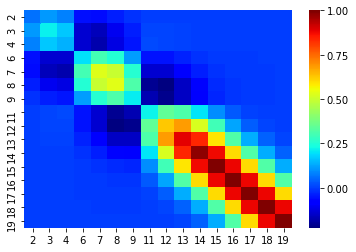
\includegraphics[width=\linewidth, height=\textheight -120pt ,keepaspectratio]{gp/post20d}
	\end{center}
	Notice that the variance of the points near the newly added data points seem to have reduced.
\end{frame}

% for cov
\forloop{iter}{1}{\value{iter} < 6}%
{%
	\begin{frame}{Conditional Multivariate (20D) Distribution Samples | Random State - \theiter}
		\begin{center}
			\includegraphics[width=\linewidth, height=\textheight -120pt ,keepaspectratio]{gp/20d/conditional/\theiter}
		\end{center}
		From the animation above, we can see points near the added data points (red) seem to have a much lower variance compared to points far off.
	\end{frame}
}

\begin{frame}{Multivariate (20D) Posterior}
	\begin{center}
		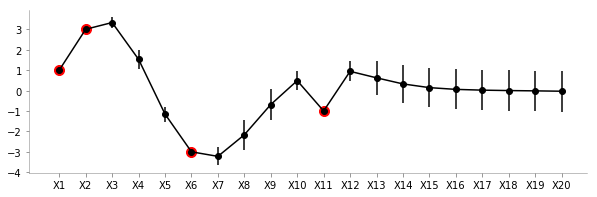
\includegraphics[width=\linewidth, height=\textheight -120pt ,keepaspectratio]{gp/20dcov} \\
	\end{center}
	We can easily see the reduced variance in this plot.
\end{frame}

\urldef\urlsek\url{http://evelinag.com/Ariadne/covarianceFunctions.html}
\section{Kernels!}
\begin{frame}{Defining Squared Exponential Kernel}
	We will now a bit into kernels. These are functions that are used to generate the covariance matrix.
	
	Below we have defined, what is known as the Squared Exponential Kernel\footnote{\urlsek}. \\
	
	We have 2 parameters the define this kernel.
	\begin{itemize}
		\item $\sigma$ is the scale of variance.
		\item $l$ is the influence of the point to the neighbouring points
	\end{itemize}

	$$
	k(x_1, x_2) = \sigma^2 \exp\left(-\frac{(x_i - x_j)^2}{2l^2}\right)
	$$
\end{frame}

\begin{frame}{Varying $l$ with $\sigma = 1$}
	\begin{center}
		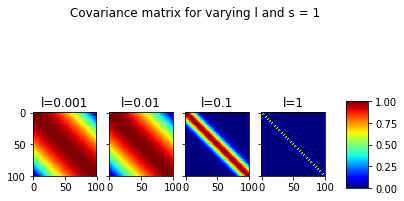
\includegraphics[width=\linewidth, height=\textheight -120pt ,keepaspectratio]{gp/vary_l}
	\end{center}
	
\end{frame}

\begin{frame}{Varying $\sigma$ with $l = 0.1$}
	\begin{center}
		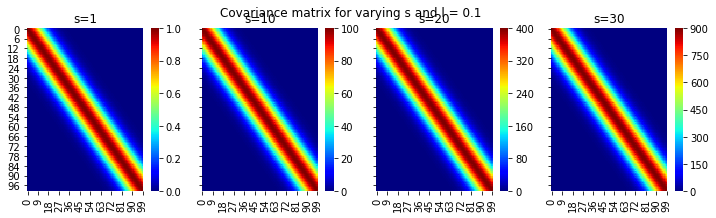
\includegraphics[width=\linewidth, height=\textheight -120pt ,keepaspectratio]{gp/vary_s}
	\end{center}
	
\end{frame}


\end{document}